%\documentclass[twoside, 12pt, finnish]{book} %dokumenttiluokka ja sille muutamia määrityksiä
\documentclass[twoside]{article}
\usepackage[hcentering,bindingoffset=20mm]{geometry}
\usepackage{lipsum}
\usepackage[utf8]{inputenc}
\usepackage{mathtools}
\usepackage{amsfonts}
\usepackage{emptypage}
\usepackage{pdfpages}
\usepackage{eurosym}
\usepackage{amsmath} %matematiikka kirjasto
\usepackage{graphicx} %kuvien liittämiseen kuten etusivun Aalto-logo
\usepackage[finnish]{babel} %suomenkieli
\addto{\captionsfinnish}{\renewcommand{\bibname}{Lähteet}}
\usepackage{amsmath} %matematiikka kirjasto
\usepackage{graphicx} %kuvien liittämiseen kuten etusivun Aalto-logo
\usepackage{cite}
\usepackage{titlesec}
\titleformat{\chapter}
{\Large\bfseries} % format
{}                % label
{0pt}             % sep
{\huge}           % before-code

\usepackage{hyperref}
\hypersetup{pdfpagemode=UseNone, pdfstartview=FitH, colorlinks=true,urlcolor=red,linkcolor=black,citecolor=black,pdftitle={Toimintakertomus},pdfauthor={Partiolippukunta Helsingin Kotkat ry}}
\setlength{\parindent}{0mm} %ei sisennystä uusiin kappaleisiin
\setlength{\emergencystretch}{15pt} %tekstin muokkaamiseen eli sallii välien venytyksen riveillä jotta näyttää paremmalta
\newcommand*{\findate}{\the\day.\the\month.\the\year} %uusi komento päivämäärän esittämiseen suomalaisittain
\renewcommand\thesection{\arabic{section}}
\usepackage{fancyhdr}
\pagestyle{fancy}
\rfoot{}
\lfoot{}
\cfoot{\thepage}
%\lhead{}
%\chead{}
%\rhead{Partiolippukunta Helsingin Kotkat}
%\renewcommand{\headrulewidth}{0.4pt}
%\renewcommand{\footrulewidth}{0.4pt}
%\renewcommand{\sectionmark}[1]{\markright{#1}}
\usepackage{caption}
\begin{document}
\includepdf{osiot/etusivu.pdf}
\cleardoublepage
\tableofcontents
\cleardoublepage
%\begin{titlepage}
	\centering
	
\includegraphics[width=0.5\textwidth]{kuvat/heko.png}\par\vspace{1cm}
	{\scshape\LARGE Partiolippukunta Helsingin Kotkat \par}
	\vspace{1cm}
	{\scshape\Large Toimintakertomus\par}
	\vspace{1.5cm}
	{\huge\bfseries 1.9.2015-31.8.2016\par}
	\vspace{2cm}
	\vfill
	\vfill
	{\large Hyväksytty yhdistyksen vuosikokouksessa 21.10.2016}
\end{titlepage}
\tableofcontents
\newpage


\section{Yleistä lippukunnasta}
\begin{figure}[htb]
	\begin{center}
		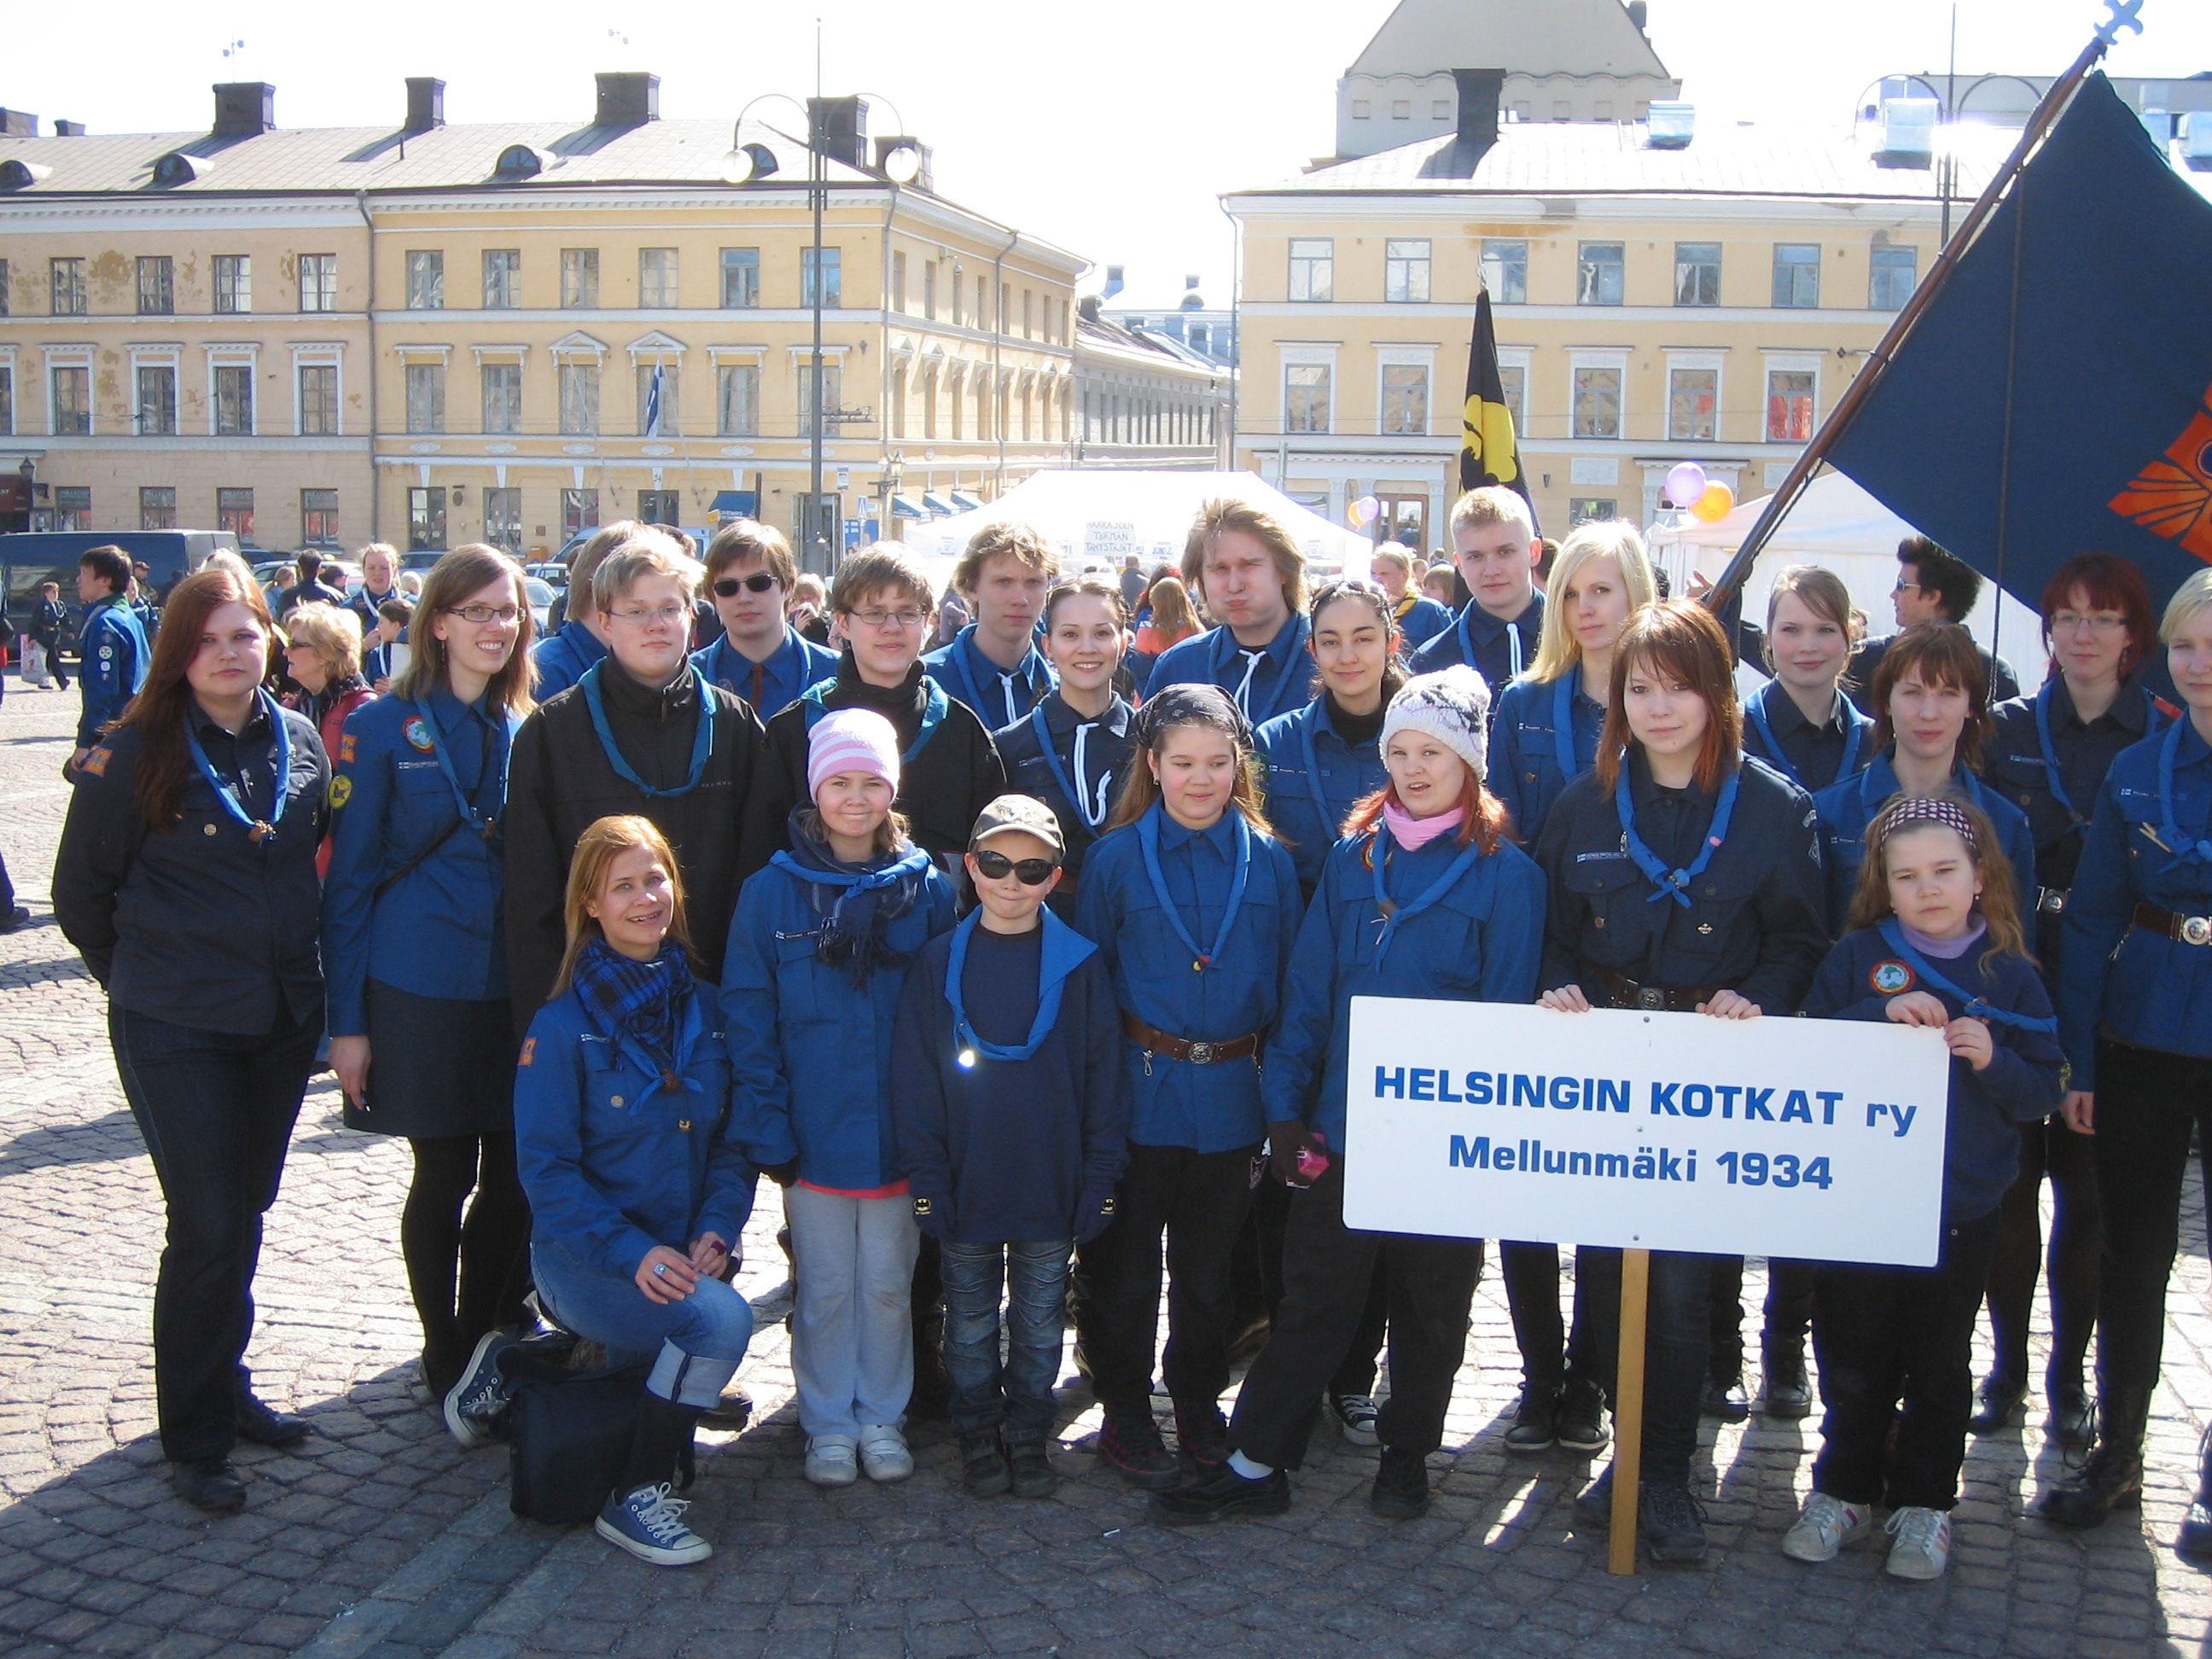
\includegraphics[height=7cm]{kuvat/paraatissa.jpg}
	\end{center}
	\captionsetup{labelformat=empty}
	%\caption{\textbf{Lippukunnan kämppä, Kyöpeli.}}
\end{figure}

Helsingin Kotkat on vuonna 1934 alunperin poikalippukunnaksi Helsingin keskustaan perustettu partiolippukunta. Myöhemmin lippukunta yhdistyi paikallisen tyttölippukunnan kanssa sekalippukunnaksi ja muutti Mellunmäkeen, jossa se toimii edelleen. Lippukunnalla on pitkät perinteet erityisesti luonnossa liikkumisessa ja partiotaitokilpailuissa. Lippukunnan pitkä ikä näkyy toiminnassa ja perinteissä ja vanhatkin, jopa jo eläkkeellä olevat jäsenet toimivat lippukunnassa edelleen aktiivisesti.\\
\\Helsingin Kotkat toteuttaa toiminnassaan Suomen Partiolaisten partio-ohjelmaa. Toiminta oli kuluneella kaudella aktiivista ja lippukunnan jäsenmäärä oli vakaa. Lippukunta osallistui aktiivisesti läheisten lippukuntien kanssa järjestettyyn yhteistoimintaan ja oli kantava voima kaupunginosansa nuorisötyössä.\\
\\Lippukunnassa toimi keväällä 2016 yksi tyttösudenpentulauma, kaksi poikasudenpentulaumaa, yksi tyttöseikkailijajoukkue, yksi poikatarpojajoukkue, yksi tyttötarpojaryhmä sekä yksi poikasamoajaryhmä. Lisäksi lippukunnan johtajatehtävisä toimivat vaeltajat ja aikuiset ovat kokoontuneet toiminnansuunnittelun merkeissä. Myös johtajahuoltoa järjestettiin, jotta johtajiston jaksaminen saatiin taattua. 
\newpage


\section{Toiminta}
\subsection{Kokoukset}

\begin{figure}[htb]
	\begin{center}
		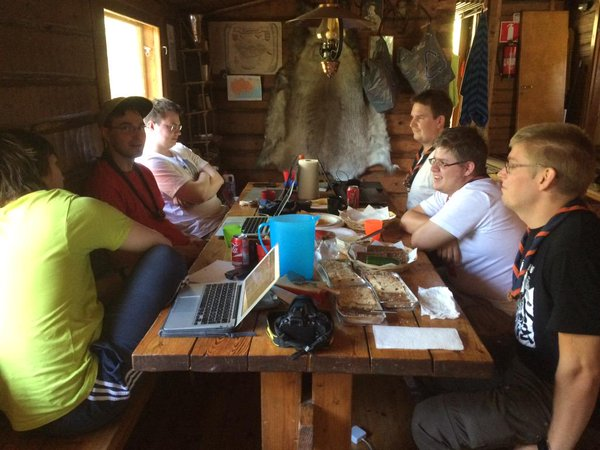
\includegraphics[height=7cm]{kuvat/kokous.jpg}
	\end{center}
	\captionsetup{labelformat=empty}
	\caption{\textbf{Toiminnansuunnittelua lippukunnan kämpällä.}}
\end{figure}


Ryhmät koontuivat omiin tapaamisiinsa viikoittain ja johtajat pitivät omia kokouksiaan tarpeen mukaan, esimerkiksi retkien suunnittelua varten. Kokouksista ja niiden määrästä lista alla:\\
\begin{center}
	\begin{tabular}{ l l }
		Vuosikokous & 1 kpl\\
		Vaalikokous & 1 kpl\\
		Hallituksen kokous & 9 kpl\\
		Poikasamoajat & 20 kpl\\
		Poikatarpojat & 20 kpl\\
		Poikasudenpennut & 50 kpl\\
		Tyttötarpojat & 25 kpl\\
		Tyttöseikkailijat & 25 kpl\\
		Tyttösudenpennut & 25 kpl\\
					 & \\
		\textbf{Yhteensä} & \textbf{176 kpl}\\
	\end{tabular}
\end{center}
Lisäksi vuoden mittaan on pidettu lukuisia muita pienempiä ja epävirallisia kokouksia, joissa on esimerkiksi suunniteltu toimintaa, retkiä tai kämppien kunnostusta.
\subsection{Leirit ja retket}
\subsubsection{Jouluretki}
Joulukuussa 2015 Helsingin Kotkat järjesti kaksi yötä kestäneen talviretki Tontun. Retkenjohtajina toimivat yhdessä Jukka Holopainen ja hänen kaksoisveljensä Pekka Holopainen. Retken teemana toimi tonttuilu ja viikonlopun aikana suunnistettiin, harjoiteltiin partio- ja kädentaitoja sekä kehitettiin lasten esiintymistaitoja. Lisäksi retkellä annettiin partiolupauksia jokaiselle ikäkaudelle. Retki oli johtajiensa PJ-lopputyö ja sille osallistui 11 johtajaa ja 26 retkeläistä.
\subsubsection{Kevätretki}
Huhtikuussa 2016 järjestettiin lippukunnan perinteinen keväretki, jonka johtajana toimi Adel Gatoui. Retkelle otettiin mukaan kaikki seikkailijat ja heitä vanhemmat HeKolaiset. Tämä johtui siitä, että retkellä ei ollut lainkaan sisämajoitusta ja siellä järjestetty pienoisvaellus oli suhteellisen pitkä. Mukana oli 9 johtajaa ja 16 retkeläistä.
\subsubsection{SuSe-leiri}
Tähän juduja kun leiri on pidetty.
\subsubsection{Roihu 2016}
Tähän setti Roihun jälkeen.
\subsubsection{Ryhmien retket}
Lippukunnan ryhmät ja osastot retkeilivät seuraavasti:
\begin{center}
	\begin{tabular}{l l l}
		16.-18.10. & Poikasamoajat Willassa & 4 osallistujaa\\
		30.10.-1.11. & Tyttöseikkailijoiden retki & 10 osallistujaa\\
		11.-13.3. & Tyttöosaston retki & 21 osallistujaa\\
	\end{tabular}
\end{center}
\subsection{Muu toiminta}
\subsubsection{Kisat}
Helsingin Kotkaista oli edustajat lähes jokaisissa pääkaupunkiseudulla järjestetyissä partiotaitokilpailussa. Mainetta ja kunniaa ei niistä kummemmin niitetty, mutta niissä edustaneiden lippukuntalaisten partiotaidot kasvoivat ja kehittyivät henkisen kasvun ja partioaatteen ymmärtämisen ohella.
\subsubsection{Kurssit ja koulutus}
Lippukuntalaiset kävivät tällä toimikaudella poikkeuksellisen paljon johtajakoulutusta. Partionjohtajakurssilla ja ryhmänohjaajakurssilla oli molemmilla kaksi edustajaa. Ryhmänohjaajakurssi järjestettiin yhteistyössä Vuosaaren Vesipääskyjen ja Sipoonkorven Haltiat. Kurssi koostui kahdesta kaupunkitapaamisesta sekä maasto- ja kämppäviikonlopuista, joista viikonloppujen aikana suoritettiin myös partionjohtajakurssin johtamisharjoitteita. Osallistujia ryhmänohjaajakurssilla oli 15.
\subsubsection{Johtajahuolto}
Lippukunnan perinteisiin kuuluu myös johtajahuollon järjestäminen. Johtajisto käy aina perinteisesti Joulun alla keilaamassa, jonka jälkeen siirrytään illalliselle läheiseen ravintolaan. Johtajahuoltoa toteutettiin myös toiminnansuunnitteluviikonloppuna Nuuksiossa elokuun lopulla.
\subsubsection{Lupauksenannot}
Tärkeä osa partiotoimintaa on sen arvojen ja aatteiden tunnustaminen ja ymmärtäminen. Tätä varten on olemassa partiolupaus, joka annetaan lupauksenantotilaisuudessa lippukunnanjohtajalle. Tällä toimikaudella niitä järjestettiin kaksi kappaletta, yksi jouluretki Tontulla ja toinen maaliskuussa lippukunnan kololla.


\newpage
\section{Viestintä}
Lippukunnan viestintäkanavia fokusoitiin ja täsmennettiin viime toimikautena huomattavasti. Uusia kanavia otettiin käyttöön täydellä pöhinällä ja siinä onnistuttiin kiitettävästi.
\subsection{Sosiaalinen media ja muut sähköiset kanavat}
\subsubsection{Facebook}
Lippukunnalla on facebook-sivu, jota kautta vanhemmille viestitään lähes viikoittain. Retkikirjeet ja muut ulospäin suunnatut tiedotteet saavuttavat kohdeyleisönsä sitä kautta erittäin ansiokkaasti. Johtajistolla ja hallituksella on myös omat yksityiset ryhmänsä, joissa keskustellaan lippukunnan asioista.
\subsubsection{Instagram}
HeKo avasi myös Instagram-tilin, jonne retkiltä ja leireiltä lähetetään kuvia toiminnasta. Lippukunnalla on oma hashtag, \#partioheko.
\subsubsection{Twitter}
Satunnaisesti lippukunta viestii myös twitterissä, joskin tämä on verrattain vähäistä muihin kanaviin nähden.
\subsubsection{heko.org}
Lippukunnan nettisivuille lisättiin huima määrä staattista informaatiota, etenkin uusia ja tulevia jäseniä varten. Sivuilla julkaistiin myös kutsut yhdistyksen kokouksiin. Sivuilla näkyy nyt myös Kyöpelin varauskalenteri ja lippukunnan oma virallinen toimintakalenteri, jotka kuka tahansa voi lisätä omaan Google-kalenteriinsa.
\subsubsection{Telegram}
Johtajisto siirtyi syksyllä 2014 käyttämään pikaviestimenään Telegramia. Tätä jatkettiin ja kehitettiin myös viime toimikaudella.
\subsection{Muut kanavat}
\subsubsection{HeKo-posti}
HeKo-postia lähetettiin aiempia vuosia vähemmän. Tämä johtui osaltaan siitä, että sähköiset viestimet ovat osaltaan syrjäyttäneet paperisena postitettavat tiedotteet.
\subsubsection{Ilmoitustaulu}
Kolon seinällä on ilmoitustaulu, jonne satunnaisesti saatetiin laittaa pieniä tiedotteita tai huomautuksia. Taululle laitettiin myös kutsut yhdistyksen kokouksiin.
\subsubsection{Jaettavat laput ja kirjeet}
Tapahtumakohtaisesti lapsille jaettiin kokouksissa mukaan kirjeitä ja tiedotteita. Tapa on vanha kuin Abraham, mutta todistetusti toimii erittäin hyvin. Tämä on myös osasyy sille, miksi HeKo-postin julkaisutiheys on vähentynyt merkittävästi.
\newpage


\section{Toimitilat}
\subsection{Kolo}
Lippukunnan pääasiallisena toimitilana, eli Kolona toimii Mellunmäki-Seuralta vuokrattu noin 50 neliömetrin kokoinen huone. Tilassa olevaa keittiötä alivuokrataan Hilkka Harjulle, joka käyttää tilaa päivisin.
\subsection{Varasto}
Lipukunnan retki- ja leirikalustoa säilytetään Sallatunturintie 1:ssä, jossa lippukunnalla on noin 30 neliömetrin kokoinen varastotila. 
\subsection{Willa}
Lippukunnan käytössä on Nuuksiossa yksityisellä luonnonsuojelualueella sijaitseva Willa-niminen kämppä. Kämpälle tehdään ryhmien toimesta retkiä muutaman kerran vuodessa. Kämpästä ei makseta vuokraa.
\newpage

\section{Kyöpeli}
\begin{figure}[htb]
	\begin{center}
		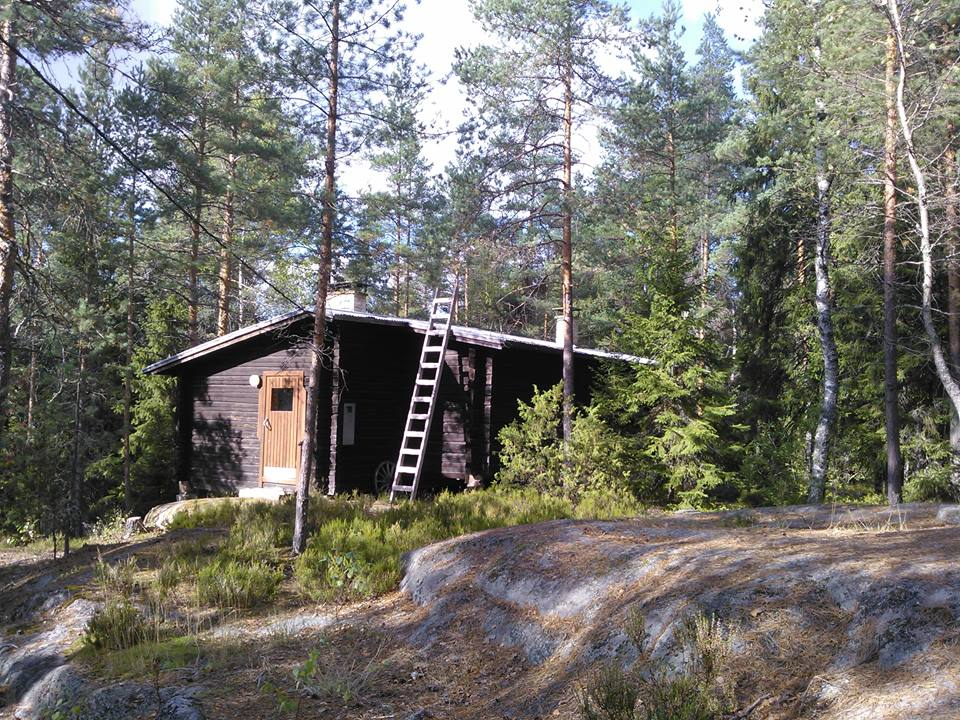
\includegraphics[height=7cm]{kuvat/kyopeli.jpg}
	\end{center}
	\captionsetup{labelformat=empty}
	\caption{\textbf{Lippukunnan kämppä, Kyöpeli.}}
\end{figure}

Lippukunnan pääasiallisena kämppänä toimii osoitteessa Ruuhijärventie 17 sijaitseva Kyöpeli. Kämppään kuuluu laajahko tontti. Kämppää käytetään lippukunnan omiin retkiin ulkopuolelle vuokrauksen lisäksi. Myös lippukunta maksaa omista retkistään vuokraa, jotta kämpän ylläpitoon saadaan riittävästi varoja.\\
\\Kämpän suhteen tehdään läheistä yhteistyötä Paakaupunkiseudun partiolaisten kanssa. Tämä näkyy siten, että lippukunnalla on 1/4-osa käyttöoikeus kaikkiin piirin tarjoamiin palveluihin. Näihin kuuluu sauna, vesikaivo ja jätehuolto.\\
\\Kyöpelillä vietetään joka vuosi talkoot, yleensä Helatorstaina. Tällä toimikaudella talkoissa tehtiin valtavat määrät puutöitä sekä uudet penkit nuotiopaikalle, lisäksi sisätiloissa tehtiin parannustöitä keittiöön.
\newpage

\newpage
\section{Jäsenet}
Lippukunnan jäsenmäärä on pysynyt vakaana (tilanne elokuu 2015)\\
\begin{center}
\begin{tabular}{ l l l }
	\textbf{Jäsenryhmä} & \textbf{Ikä} & \textbf{Määrä}\\
	Sudenpennut & 7-9 & 8\\
	Seikkailijat & 10-12 & 17\\
	Tarpojat & 13-15 & 18\\
	Samoajat & 15-17 & 3\\
	Vaeltajat & 18-22 & 13\\
	Aktiiviset aikuiset & 23-29 & 8\\
	Muut aikuisjäsenet & 30+ & 20\\
				   & & \\
	\textbf{Jäsenet yhteensä} & & \textbf{87}
\end{tabular}
\begin{figure}[htb]
	\begin{center}
		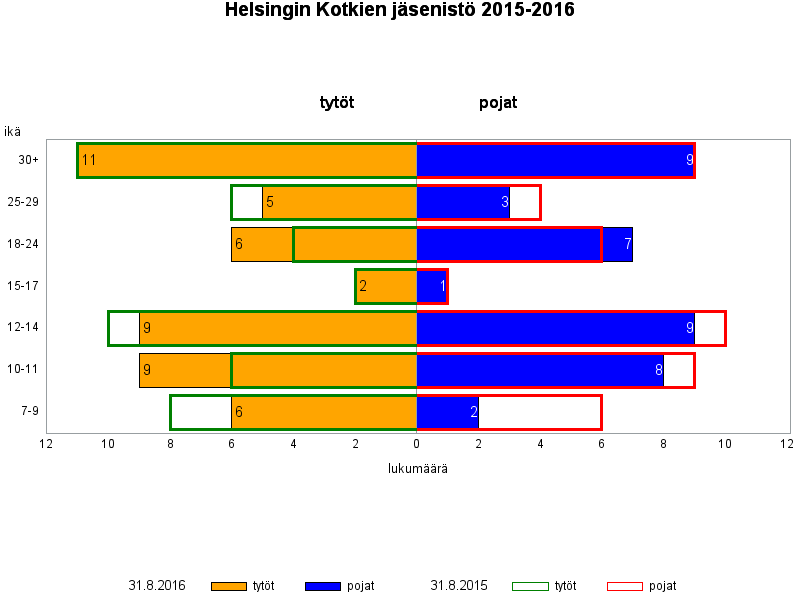
\includegraphics[height=10cm]{kuvat/jasenet.png}
	\end{center}
	%\caption*{\textbf{Jäsentilanne kesäkuussa 2016.}}
\end{figure}


\end{center}

\section{Hallitus ja toimihenkilöt}
\begin{center}
	\begin{tabular}{ l l }
		\textbf{Hallitus} & \\
		Onni Lampi & lippukunnanjohtaja\\
		Hanna Tompuri & lippukunnanjohtajan apulainen\\
		Pyry Aaltonen & sihteeri, uudet jäsenet\\
		Eero Lilja & taloudenhoitaja, jäsenrekisterinhoitaja\\
		Pekka Holopainen & varasto- ja kolovastaava\\
		Heidi Ekblom & koulutusvastaava, viestintämestari\\
		Pauli Saarikoski & ohjelmavastaava\\
		Aapo Launiainen & kämppävastaava\\
						     & \\
		\textbf{Muut toimihenkilöt} & \\
		Kimmo Huurinainen & kirjanpitäjä\\
		Ari Söderqvist & toiminnantarkastaja\\
		Minna Söderqvist & varatoiminnantarkastaja\\
							      & \\
		\textbf{Ryhmät ja niiden johtajat} & \\
		Uudet poikasudenpennut & Ikra Sheikh, Jenni Halkola, Tanja Kaappola\\
		Vanhat poikasudenpennut & Hanna Tompuri, Heidi Ekblom\\
		Poikatarpojat & Pauli Saarikosi, Pyry Aaltonen\\
		Tyttöseikkailijat & Ikra Sheikh, Jenni Halkola, Tanja Kaappola\\
		Poikasamoajat & Adel Gatoui\\
		Tyttösudenpennut & Mari Aho\\
		Tyttötarpojat & Aino Pirskanen, Elli Kasvi\\
	\end{tabular}
\end{center}



\newpage
\section{Talous}
Lippukunta on säilynyt vakavaraisena läpi tilikauden. Lippukunta sai Urlus-säätiöltä 5000\euro{} avustusta Kyöpelin katon uusimiseen, tämä toteutetaan alkuvuodesta 2017. Lippukunta haki ja sai myös 1500\euro{} rahaa leirikalustonsa uusimiseen, tällä hankittiin uusi puolijoukkueteltta. Varoja koitetaan säästää tulevaisuutta varten, esimerkiksi suojaamaan nousevalta toimitilavuokralta.\\
\\Varainhankintaa toteutettiin perinteisin keinoin. Näihin kuuluivat esimerkiksi adventtikalentereiden myyminen sekä osallistuminen Lions Clubin ja Mellunmäki-seuran tapahtumiin.\\
\\Kyöpelin suhteen varoja kerätään aktiivisesti vuokratuloilla. Vuokratulot käytetään pääsääntöisesti kiinteistön kunnostamiseen ja muihin huoltotoimenpiteisiin. Lippukunta sai myös 5000\euro{} suuruisen summan osana Haapakerttujen viime vuotista lahjakirjaa. Viimeisenä mainittu summa on korvamerkitty Kyöpeliä varten, eikä siihen kosketa ilman lippukunnan hallituksen erillistä päätöstä.



\newpage
\section{Taustayhteisöt}
\begin{figure}[htb]
	\begin{center}
		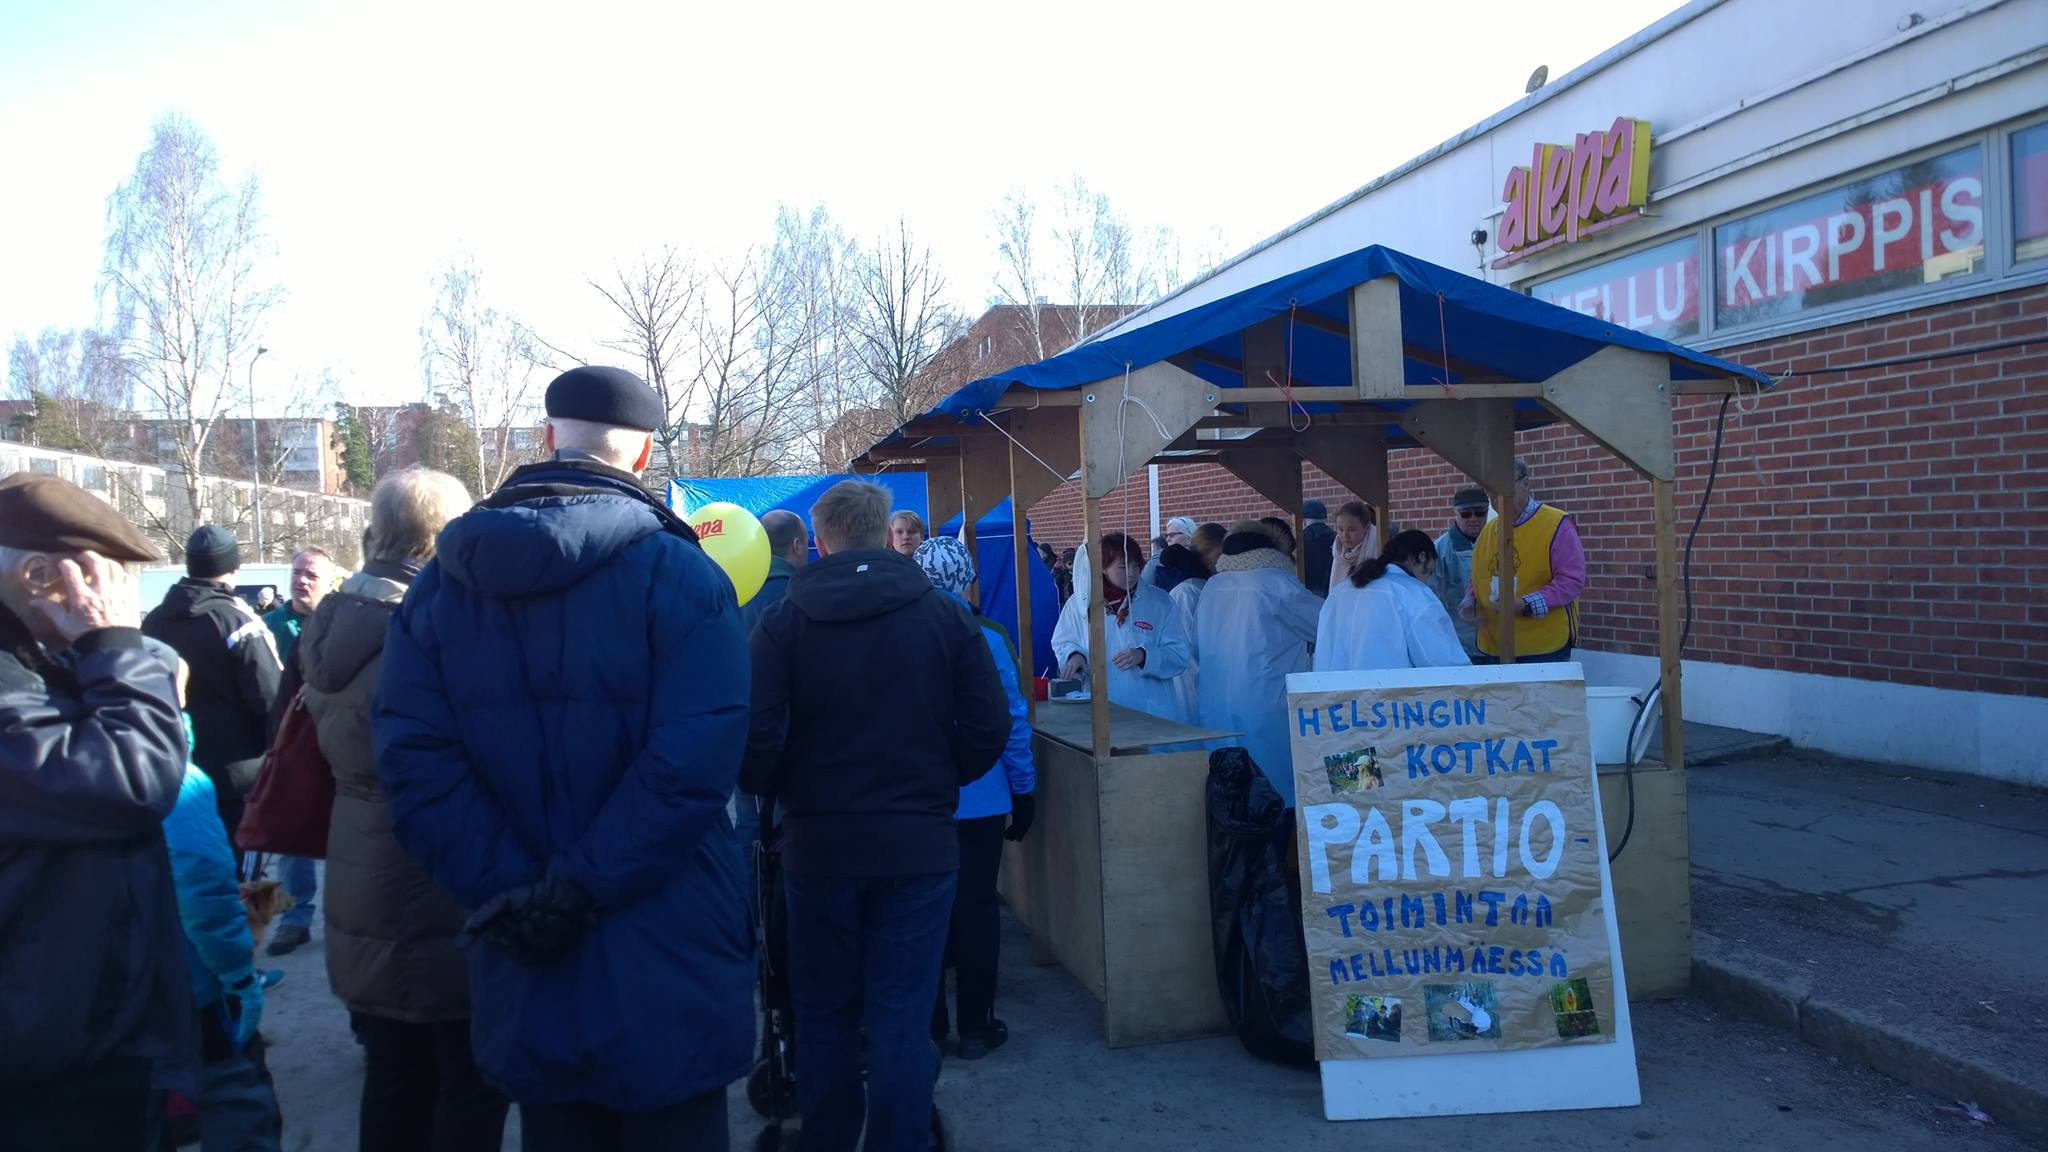
\includegraphics[height=7cm]{kuvat/lettukestit.jpg}
	\end{center}
	\captionsetup{labelformat=empty}
	\caption{\textbf{Vohvelimyyntiä Mellunmäen Lionsien kevätriehassa.}}
\end{figure}

Taustayhteisöinä ovat tuttuun tapaan toimineet Mikaelin seurakunta, Mellunmäen Lions Club ja Partiolippukunta Helsingin Kotkat ry:n Venhempainyhdistys ry. Jokaiseen taustayhteisöön on oltu aktiivisesti yhteydessä ja heidän kanssaan on järjestetty tapahtumia.\\
\\Lippukunta oli useaan otteeseen mukana auttamassa Mikaelin seurakunnan tapahtumissa keräämällä mm. kolehtia ja nostamalla lipun itsenäisyyspäivänä. Yhteistyö Mellunmäen Lions Clubin kanssa rajoittui lähinnä avustamiseen kevätriehassa ja itsenäisyyspäivän lipunnostoon Mellunmäen ostoskeskuksen edustalla, mutta yhteydenpito oli silti erittäin aktiivista ja molemmin puolin vallitsi herrasmiessopimus siitä, että apua annetaan tarvittaessa puolin ja toisin.\\
\\Vanhempainyhdistys oli tuttuun tapaansa todella tärkeässä asemassa lippukunnan toiminnan kannalta, sen kanssa järjestettiin Kyöpelin talkoot sekä keväinen iltapäiväretki jätelaitokselle. 


\newpage\null\thispagestyle{empty}\newpage
\newpage\null\thispagestyle{empty}\newpage
\end{document}
